\chapter{Introduction}
\label{cha:introduction}

The world's population is growing each year. 
In order to raise to the challenges that arise with a growing population, it is of great importance that healthcare is made to be more efficient and robust.
One way of increasing the efficiency as well as the quality of healthcare is to create automated systems that can aid doctors in their process.
As the population grows, it is of utmost importance to ensure that the quality of diagnoses remain high, and that the risk of missing some critical piece of information is minimized.
Taking advantage of the available medical information is key to create such systems.

Most of the approaches that exists today to create the aforementioned automated systems need a set of categorized data in order to identify and exploit certain patterns.
The purpose of this thesis is to evaluate different techniques for labeling multi-label clinical reports.
The goal is to make the set of labeled reports more useful in future systems by labeling them based on a strategy instead of selecting them at random.
By using a selection strategy, the need for a large set of labeled reports could be reduced.
The work is done at Sectra Medical Imaging IT Solutions AB in connection with a research project they have with Region Skåne.
Region Skåne is responsible for the healthcare in Skåne, the southern most county of Sweden.
This research project works on investigating how to use machine learning and text mining techniques to improve the functionality of their products and aid the physicians in their work.

\section{Motivation}
\label{sec:motivation}

Information pertaining to a patient's diagnosis is often in the form of written clinical reports.
This is a good example of data that can be utilized in automated systems.
By extracting information from old reports, the process of writing new ones can be simplified.
A system could show cases with similar features as the one currently being written, the doctor could then compare the findings and check if they have obtained an abnormal result.
Being able to perform such a comparison will result in extra quality assurance in the diagnostic flow.
It could also provide doctors with more confidence in that their diagnosis is correct.

The problem systems like this would face is to categorize medical reports in order to make further suggestions.
One approach that is commonly used for such problems is machine learning, which is a field where a set of inputs is used to create a mapping to some output values~\cite{bishop2006pattern}.
This is done by using data to build a, usually statistical, model.

The task of predicting a category, or class, for a given text document is called text classification.
Text classification is usually solved using supervised learning~\cite{aggarwal2012surveyclass}. 
In supervised classification, there exists a set of inputs, in this case text data, that already have a category assigned to them.
This data is then used to fit the model so that it later can make predictions for inputs that it has not yet been exposed to.
Some models that have been shown to be successful in text classification are Neural Networks, Bayesian Classifiers, Decision Trees and Support Vector Machines (SVM)~\cite{aggarwal2012surveyclass,joachims1998text, aggarwal2012surveyclass, tong2001support}.

In order to fit a machine learning model to predict categories for clinical reports, we need a set of already categorized data.
That is, categories need to be assigned to an existing set of clinical reports.
It is often the case that text data is widely available.
Coming by data that is already categorized is on the other hand much harder.
Obtaining high quality data is important for use in machine learning systems, both in healthcare and in other areas.

Since the models require a sufficient amount of categorized reports, the task of categorizing them can be cumbersome.
Improving the categorization is especially important in the case of clinical data, since doctors and other clinicians time is both valuable and limited.
By improving the process and the quality of data to be labeled, and thereby reducing the number of reports that need to be categorized, they can spend more time doing their job.

Assigning categories to reports is often referred to as labeling.
A field within machine learning that is focused on the task of improving the data labeling process is called active learning~\cite{settles2012active}.
It is a form of semi-supervised learning.
The algorithm queries an oracle (in this case a doctor) for labels for the data points that it thinks will help the model improve the most.
An overview of the components in an active learning system can be seen in Figure~\ref{fig:active-learning-model}.
This is used when there is plenty of readily available data, but assigning labels is expensive.
Since the data points to be labeled are actively selected, the model can require fewer examples than if they were selected at random.
The points can be selected by considering the certainty of the models, and request to label the documents that the model is less certain about.
Another approach, which has not been given as much attention, is using the underlying structure of the data to select points.
The goal with this approach is to capture the distribution of the categories by applying techniques such as clustering.

\begin{figure}
    \centering
    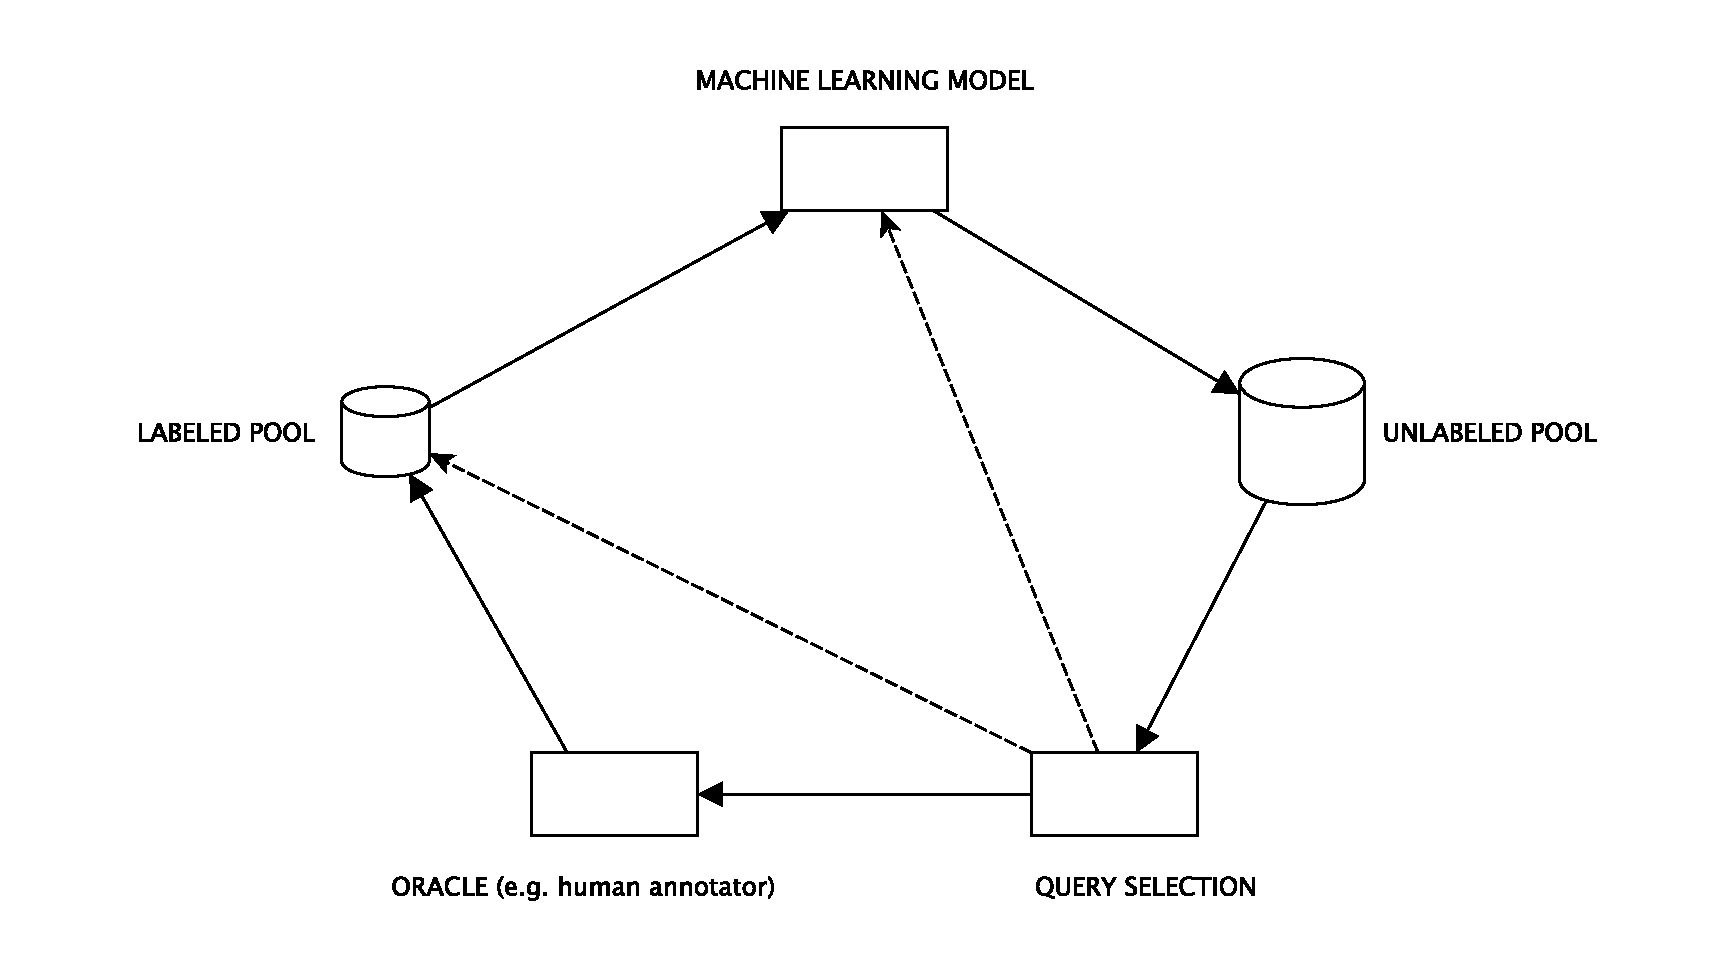
\includegraphics[width=\textwidth]{figures/active-learning-model.eps}
    \caption{An overview of an active learning system. 
    The dotted lines represents components that sampling strategies can base their calculations on.}
    \label{fig:active-learning-model}
\end{figure}

If one of two categories is assigned to each document, it is called a binary classification problem~\cite{bishop2006pattern}.
Problems where one of several classes is assigned to an instance are called a multi-class classification problem.
Multi-labeled classification is when one or more categories are assigned to each document.
This thesis is mainly concerned with the multi-label case.
Assigning several categories to a document is more time consuming than in the cases where only one option needs to be identified.
In those cases the process can be stopped when the appropriate category has been found.
However, when a document can be assigned several categories, the entirety of the text needs to be considered.
For example, a news article can be on several subjects, such as both economics and sport.
Even when the category sport has already been identified, the rest of the document still has to be read in order to find any additional categories.
Using active learning to enhance the labeling of documents is therefore even more useful in the multi-labeled case, since the cost of labeling the individual reports is higher.

\section{Aim}
\label{sec:aim}

The purpose with this thesis project is to evaluate different active learning techniques that can be used to increase the quality of the labeled reports.
Increasing the quality of the reports will also reduce the need for a large set of labeled reports within the project.
Resulting from this will be a complete, standalone, system for labeling reports.
The reports are interactively queried so a user can label the ones that are deemed most useful by the system.
Labeling data to use in machine learning will probably be necessary for a long time ahead, but the aim here is to create a system that makes it more efficient.
The technique chosen will then be integrated with an existing web interface that Sectra created for the purpose of labeling reports.
This interface can be seen in Figure~\ref{fig:web-interface}.

\begin{figure}
      \centering
      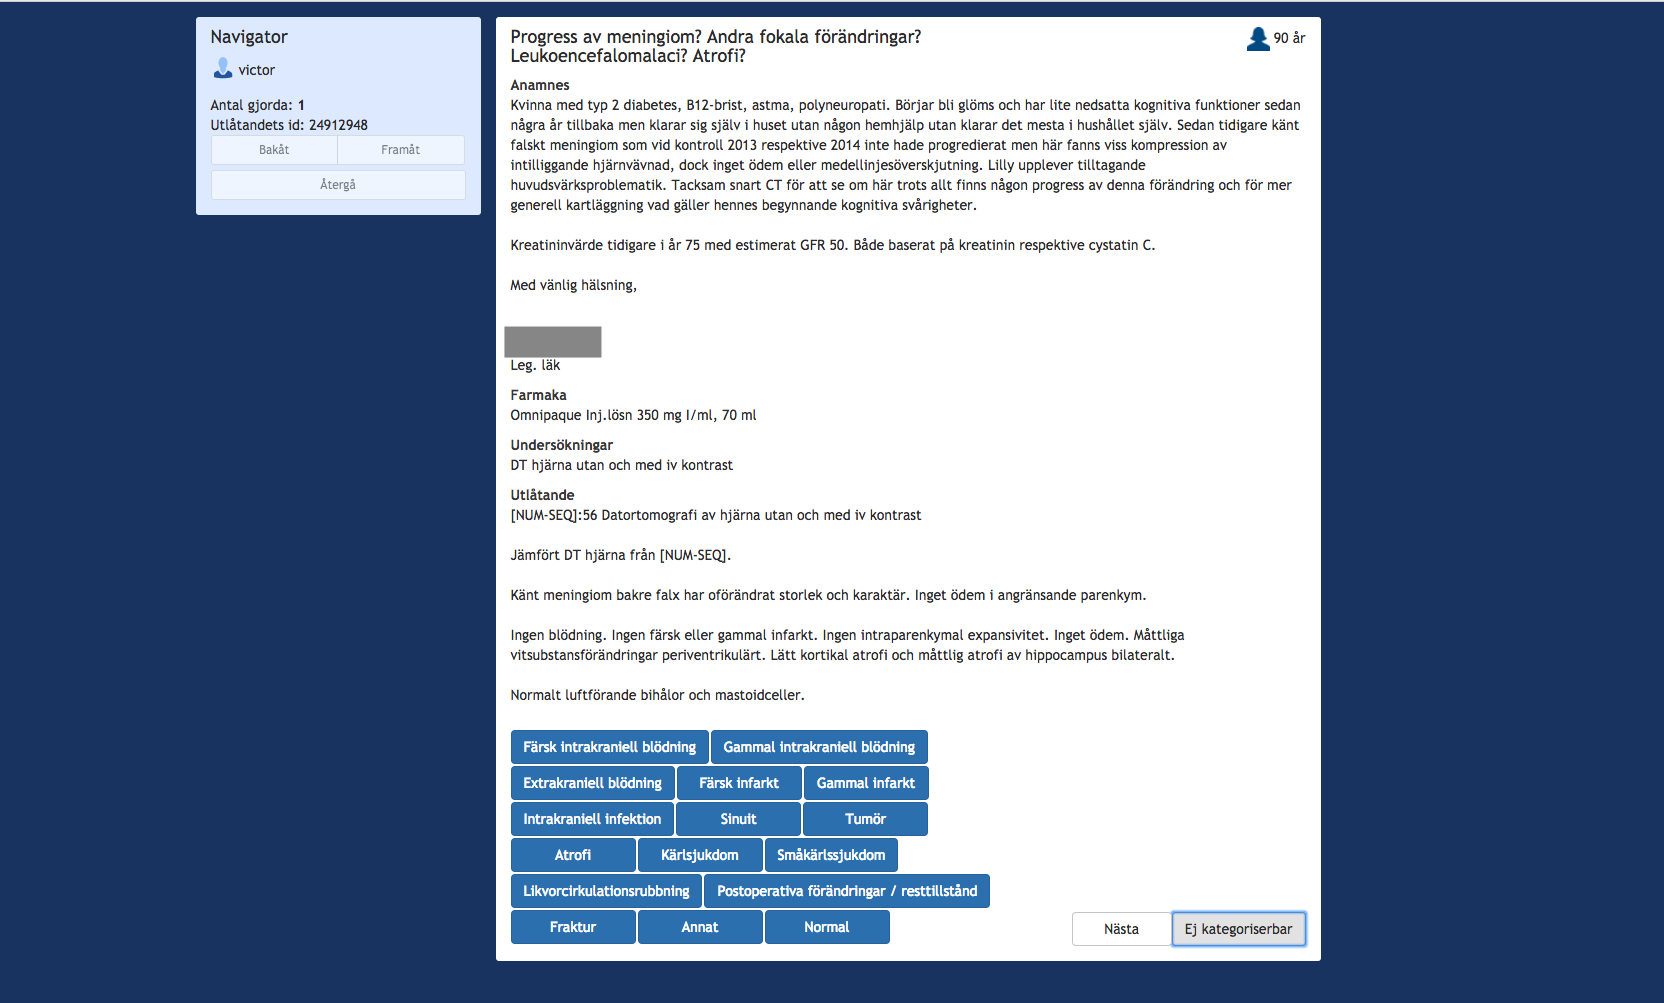
\includegraphics[width=\textwidth]{web-interface}
      \caption{A screenshot of the interface used to label clinical reports at Sectra. 
               A report is presented to the user, who can then select whichever categories (the blue buttons) deemed appropriate.
               By pressing ``next'', the system presents a new reports.}
      \label{fig:web-interface}
\end{figure}

In the work that they have done so far in the research project a doctor has labeled an initial set of reports.
This was done by simply selecting the reports in the order they were on file.
The doctor that primarily worked with the labeling stated that the distribution over the labeled categories was very skewed.
The vast majority of labeled documents were assigned to a small subset of the categories.
A skewed dataset causes the number of clinical reports that need to be labeled to increase a lot.
For a statistical model to be able to achieve good results with the less frequently occurring categories, a large number of reports needs to be labeled in order to obtain a good amount of reports with these categories.
Obtaining a more balanced dataset is desirable.

In addition to this, the doctors came up with a new set of labels that were to be used.
So the sampling strategies have to work from a non-existent, or very small, initial set of labeled reports.

\section{Research questions}
\label{sec:research-questions}

The specific research questions that this thesis treat are presented here.
They are the primary focus of study.
There are two main research questions, both of which relate to active learning.
In addition to this, a question regarding how to remove reports that do not need to be labeled is treated as well.

The clinical reports are of a multi-label nature, and how we are choosing the documents to be sampled is important.
Three different sampling strategies for active learning are evaluated for this purpose.
These are: binary version space minimization, maximum loss reduction with maximum confidence and adaptive active learning.
Their properties will be described in Chapter~\ref{cha:theory}, and a motivation behind the choice of strategies will be made in Chapter~\ref{cha:discussion}.
The algorithms to be evaluated will be based on the models certainty, as well as taking advantage of the underlying structure of the data through clustering.
The first two questions treats the evaluation of the different strategies.

\begin{enumerate}
      \item \label{intro:re-q1} 
      \textit{How well does a machine learning model perform on the labeled data set created based on the sampling strategies, given the constraints of the project?}
      \newline
      If the decision boundaries of the models can be used to pick documents that would be more informative for the model, the number of labeled documents could hopefully be reduced while still obtaining the same performance.
      When choosing the algorithm to use in the final system, there are several different constraints that will affect the final results, and therefore need to be taken into consideration.
      The number of initial reports needed for the strategies need to perform well, and the how many labeled samples need to be acquired to achieve good results will therefore be taken into account.
      In this regard, the strategies will be evaluated based on how well an SVM model perform on the data provided by them.
      This evaluation will be based on the accuracy, precision, recall and $F_1$-score of the model.
      The labeling application is running on limited hardware, so the time it takes to run the strategies will also be evaluated.

      \item \label{intro:re-q2}
      \textit{How do the the strategies affect the balance of labels in the labeled dataset?}
      \newline
      Another indication on the quality of the labeled reports is the balance between the classes.
      Based on the initially categorized clinical data, the underlying distribution of categories is far from uniform.
      There are certain categories, like the one describing that everything is okay with the patient, that are a lot more common than other more rare illnesses.

      If the dataset that is being sampled is skewed, i.e. some categories are a more frequent than others, our labeled set will likely follow that distribution.
      This will result in models requiring a lot of labeled documents to gather a sufficient amount of reports that are of the less common categories.
      Without these, the model will only perform well on the frequently occurring categories.
      Even though the original data may be imbalanced, selecting samples that contain a better balance between the different categories could improve the performance of the models.
      When a training set is imbalanced, the standard learning algorithms' performance can be significantly reduced~\cite{he2009learning}.
      The goal here is to see which one of the different sampling techniques that will result in the best balance between the different categories in the resulting dataset.

\end{enumerate}

In addition to this, after exploring the data it became clear that a substantial amount of reports state that an examination did not occur.
There was no standard format to these, but their subject matter was very similar.
The third research question treats whether or not these reports can be filtered out using unsupervised machine learning techniques.

\begin{enumerate}
      \setcounter{enumi}{2}
      \item \label{intro:re-q3}
      \textit{To what degree is it possible to filter out invalid clinical reports by using an unsupervised technique such as topic modeling?}
      \newline
      In the dataset from Sectra, there are reports describing patients not showing up for, or changing the time of their appointments, deceased patients or patients that have been ordered to go to another hospital.
      These reports do not contain any information of value from a medical point of view and should be discarded in the labeling process.

      Unsupervised machine learning models such as topic modeling do by definition not require any labeled documents to train on.
      If it is possible to, without any such data, to capture the necessary variance and group these invalid reports together and they can be removed from the labeling process before a doctor is presented with them.
      That would result in an additional hurdle being removed from the process.
      The filtering of reports will be evaluated using  accuracy, precision, recall and $F_1$-score.
\end{enumerate}

\section{Delimitations}
\label{sec:delimitations}

The active learning techniques will be evaluated on the publicly available Reuters-21578 \footnote{Reuters-21578, https://archive.ics.uci.edu/ml/datasets/reuters-21578+text+categorization+collection} dataset.
Even though the sampling strategies are evaluated objectively on this, the applicability of the techniques on clinical data is only evaluated by one physician.
That part of the study is therefore inherently subjective.
Another limitation to this evaluation is that it is performed on the dataset provided by Sectra, which is not available for public use, so any conclusions drawn from it may not be applicable in other scenarios.

\section{Structure of the Report}
\label{sec:structure}

Chapter~\ref{cha:theory} covers the theory behind the different active learning strategies used, as well as some techniques used for classification and processing of text.
After this, the data and an analysis of it is described in chapter~\ref{cha:data}, which is followed by Chapter~\ref{cha:experiments}, where the different experiments as well as their results are presented.
The method and results of the experiments are then discussed in Chapter~\ref{cha:discussion}.
Finally, Chapter~\ref{cha:conclusion} presents the conclusions and answers the research questions.
